\section{Разделение выборки на обучающую, валидационную и тестовую.}
\label{sec:purpose}

Одним из важных этапов разработки нейронных сетей с учителем является разделение выборки данных. Дело в том, что изначально, пришедшие данные, на которых будет обучаться нейронная сеть, представляют собой довольной сырой набор данных, которые не позволяют в полной мере сказать, что именно эти данных из себя представляют. Важными этапами являются такие шаги как разметка этих данных - т.е. определение, к какому классу объектов относится определённый набор данных и последующее разделение этих данных на выборки.

Если в случае с разметкой классов всё в большей степени понятно, то встаёт вопрос о том, какую цель преследует разбиение данных на выборки? Ответ на данный вопрос будет дан далее, что позволит оценить преимущество подхода разделения входных данных на выборки.

В машинном обучении общей задачей является изучение и построение алгоритмов, которые могут учиться и делать прогнозы на основе данных. Такие алгоритмы работают, делая управляемые данными прогнозы или решения, путем построения математической модели из входных данных.

Данные, используемые для построения окончательной модели, обычно поступают из нескольких наборов данных. В частности, три набора данных обычно используются на разных этапах создания модели.

\subsection{Обучающая выборка}

Модель изначально помещается в обучающий набор данных, который представляет собой набор примеров, используемых для соответствия параметрам модели. Модель (например, нейронная сеть) обучается на наборе обучающих данных с использованием контролируемого метода обучения (например, градиентного спуска или стохастического градиентного спуска). На практике обучающий набор данных часто состоит из пар входного вектора (или скаляра) и соответствующего выходного вектора (или скаляра), который обычно обозначается как цель (или метка). \cite{tdt}.

Текущая модель запускается с набором обучающих данных и выдает результат, который затем сравнивается с целью, для каждого входного вектора в наборе обучающих данных. На основании результатов сравнения и используемого алгоритма обучения параметры модели корректируются. Подгонка модели может включать как выбор переменных, так и оценку параметров.

\subsection{Валидационная выборка}

Затем подобранная модель используется для прогнозирования ответов на наблюдения во втором наборе данных, называемом набором проверочных данных. Набор данных проверки обеспечивает беспристрастную оценку соответствия модели учебному набору данных при настройке гиперпараметров модели (например, количество скрытых единиц в нейронной сети). Наборы данных проверки могут быть использованы для регуляризации путем ранней остановки: прекратите обучение, когда ошибка в наборе данных проверки увеличивается, так как это является признаком переобучения. Эта простая процедура на практике усложняется тем фактом, что ошибка набора данных может колебаться во время обучения, создавая несколько локальных минимумов.

\subsection{Тестовая выборка}

Наконец, тестовый набор данных представляет собой набор данных, используемый для обеспечения объективной оценки окончательного соответствия модели учебному набору данных. Если данные в наборе тестовых данных никогда не использовались при обучении (например, при кросс-валидации), набор тестовых данных также называется "holdout dataset".

\subsection{Разделение на выборки}

Далее рассмотрим пример разбиения на выборки, для последующего их использования:

\begin{itemize}
	\item 70\% train, 15\% val, 15\% test;
	\item 80\% train, 10\% val, 10\% test;
	\item 60\% train, 20\% val, 20\% test.
\end{itemize}

\begin{figure}[h]
\centering
	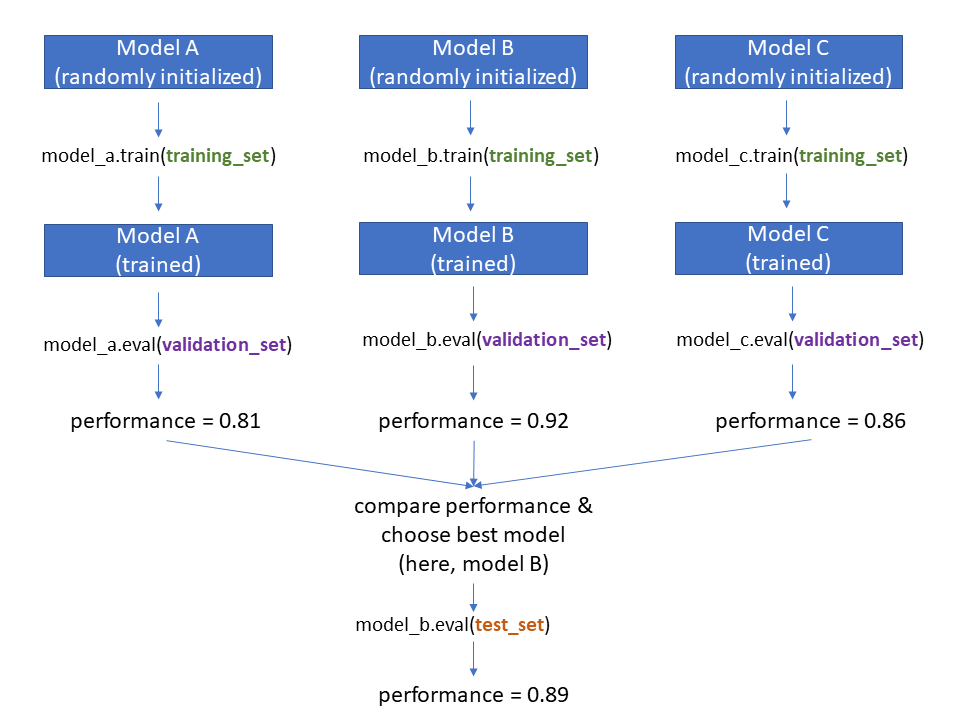
\includegraphics[totalheight=12cm]{ratio-diagram.png}
	\caption{Использование делений на выборки}
	\label{sec:purpose:payings}
\end{figure}

Как показано на рисунке, давайте представим, что у нас есть три модели для рассмотрения: модель A, модель B и модель C. Это могут быть модели с разными архитектурами, или они могут быть разными вариантами одной модели. Применим к каждой модели следующие шаги:

\begin{itemize}
	\item Случайная инициализация модели;
	\item Тренировка модели на обучающей выборке;
	\item Оценка модели на валидационной выборке;
	\item Выбор наилучшей модели на основе результатов;
	\item Оценка модели на тестовой выборке.
\end{itemize}

Почему же нельзя просто использовать один набор данных? Давайте представим, что произойдет, если использовать все данные в качестве обучающей выборки. В случае оценки работы модели, оценивалась бы только работа модели на обучающей выборке. Теперь производительность обучающей выборки может отражать то, как модель будет работать с данными, которых она никогда не видела раньше. Но в плохом случае, модель просто запомнит примеры обучающих данных, и когда мы подадим ей пример, которого она никогда не видела, произойдёт неудача, т.к. модель переобучилась ("overfitting").

В данном случае нет возможности выяснить, везет ли нам или нет, и именно поэтому необходим набор для проверки работы модели. Валидационная выборка состоит из примеров, которые модель никогда не видела при обучении, поэтому, в случае хорошего результата на валидационной выборке, можно быть более уверенным, что модель получила полезные обобщаемые принципы.

Однако встаёт вопрос - для чего необходимо наличие и валидационной и тестовой выборки одновременно? Тестовая выборка важна, потому что во время выбора наилучшей модели может опять же возникнуть "overfitting". Рассмотрим это так: допустим, были опробованы тысячи различных моделей или вариантов моделей, и были найдено оптимальные параметры для всех из них. Выбор модели с наилучшими характеристиками на валидационной выборке по своей сути означает что человек, выбравший определённую модель, настроил её на определённые значения. Точность модели, которая будет получена, по сути, будет завышена. Чтобы получить более точную и надёжную оценку того, насколько хороша эта "лучшая модель" будет работать с данными, которых она никогда не видела прежде, необходимо использовать больше данных, которых она никогда не видела раньше. Это и есть тестовая выборка. Точность на тестовой выборке, как правило, будет немного ниже, чем точность на валидационной выборке. \cite{tdt2}

Тогда встаёт вопрос о том, в каком соотношении нужно разделять выборки. Т.к. в идеале, хорошо бы иметь достаточное количество данных для каждой выборки, рассмотрим выгоду от каждой:

\begin{itemize}
	\item Больше данных в обучающей выборке будет положительно влиять на конечный результат, т.к. модель сможет найти лучшее решение для подаваемых на вход значений, следовательно - лучше решает поставленную задачу. Если же обучающая выборка имеет небольшой размер,модель не сможет нормально обучиться и следовательно, будет иметь плохую точность.
	\item Больше данных для валидационной выборки так же влияет положительно, потому что это помогает принять лучшее решение о том, какая модель является "лучшей".
	\item Больше данных для тестовой выборки так же будет положительно сказываться, потому что это даст лучшее представление о том, насколько хорошо модель работает на данных, которые она раньше не видела.
\end{itemize}

В общем виде, можно сказать, что деление на выборки должно происходить в зависимости от, например, количества данных, которые имеются в распоряжении. Например, на небольших наборах данных, можно использовать некоторые ранее рассмотренные схемы - 70-15-15, 80-10-10, 60-20-20 и т.д. Основным принципом является то, что большая часть данных должна приходится на обучающую выборку. Однако, стоит отметить и подход, применяемый для больших наборов данных, так, например, есть смысл использовать схему 98-1-1 на достаточно больших наборах данных, т.к. даже 1 процента для валидационной и 1 процента для тестовой может вполне хватить, для настройки модели и проверки её точности. Так же, вполне возможно схемы вроде 98-1,5-0,5 и 99-0,5-0,5, но только в случаях больших наборов данных. Данный выбор схемы, обычно, ложится на плечи инженера, создающего модели и конкретные ситуации.


\section{Баланс разброса и смещения}

В моделях обучения с учителем алгоритм обучается на основе известных помеченных входных данных.

Целью любого обучения с учителем является наилучшая оценка функции (f) для выходной переменной (Y) с учетом входных данных (X). Функция-решение часто называется целевой функцией, потому что это та функция, которую данная модель машинного обучения стремится аппроксимировать.

Ошибка предсказания для любого алгоритма машинного обучения может быть разбита на две части:

\begin{itemize}
	\item bias error;
	\item variance error.
\end{itemize}

\subsection{Bias error}

Bias - это упрощающие предположения, сделанные моделью для облегчения изучения целевой функции.

В общем случае, линейные алгоритмы имеют большое значение bias, что делает их быстрыми для изучения и более простыми для понимания, но в целом менее гибкими. В свою очередь, они имеют более низкую прогнозирующую производительность по сложным задачам.

\begin{figure}[h]
\centering
	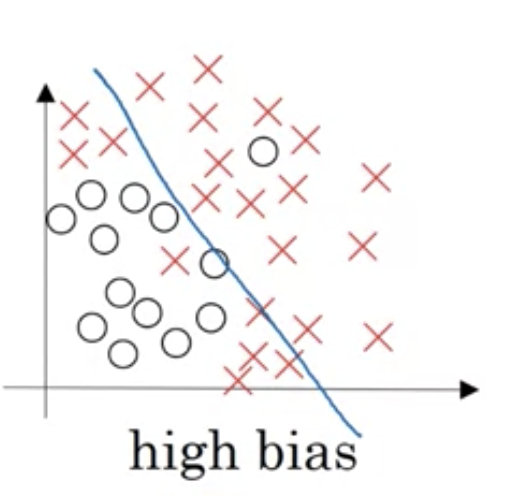
\includegraphics[totalheight=7cm]{high-bias.png}
	\caption{Пример с high bias}
	\label{sec:purpose:payings}
\end{figure}

\subsection{Variance error}

Variance - это величина, на которую изменится оценка целевой функции, если использовались разные обучающие данные.

Целевая функция оценивается по данным обучения с помощью алгоритма машинного обучения, поэтому следует ожидать, что алгоритм будет иметь некоторую дисперсию. В идеале, он не должен слишком сильно меняться от одного обучающего набора данных к следующему, что означает, что алгоритм хорош в выделении скрытого базового отображения между входными и выходными переменными.

Алгоритмы машинного обучения, которые имеют высокую дисперсию, сильно зависят от специфики данных обучения. Это означает, что специфика обучения влияет на количество и типы параметров, используемых для характеристики функции отображения. \cite{bv}

\begin{figure}[h]
\centering
	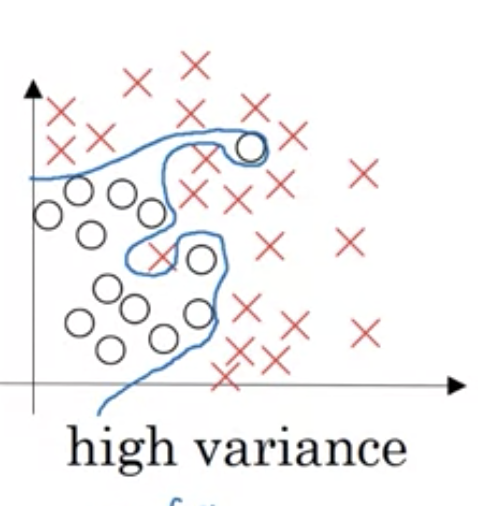
\includegraphics[totalheight=7cm]{high-variance.png}
	\caption{Пример с high variance}
	\label{sec:purpose:payings}
\end{figure}

\subsection{Баланс bias и variance}

Целью любого обучения с учителем является достижение низких показателей bias и variance. Также, в свою очередь, алгоритм должен обеспечивать необходимую точность прогнозирования с минимальными значениями разброса и смещения. Таким образом возникает задача нахождения оптимальных параметров, которые будут удовлетворять всем описанным выше критериям.

Можно отметить что:

\begin{itemize}
	\item линейный алгоритмы машинного обучения чаще имеют high bias, но в то же время low variance;
	\item нелинейные алгоритмы машинного обучения же чаще наоборот - low bias и high variance.
\end{itemize}

Идеальным сочетанием будет является нахождения точки обучения как на следующем рисунке:

\begin{figure}[h]
\centering
	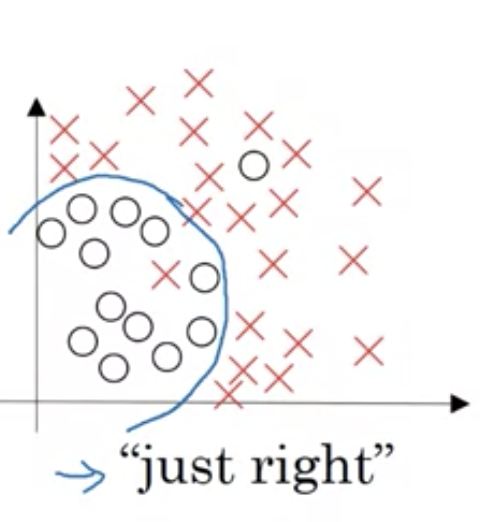
\includegraphics[totalheight=7cm]{just-right.png}
	\caption{Пример "идеально" обученной модели}
	\label{sec:purpose:payings}
\end{figure}

Также можно отметить, что предположения о наличии high bias или high variance можно делать исходя из значения ошибок на выборках. К примеру, значения ошибки на обучающей выборке в 1\% и 11\% на валидационной, может сказать, что это проявление переобучения модели, т.е. high variance. в то же время значения 15\% и 16\% на обучающей и валидационной выборках, соответсвенно, говорят о high bias. Также, может быть случай одновременного наличия high bias и high variance (например 15\% и 30\% на обучающей и валидационной выборках соответсвенно). \cite{ang}

Для решения проблем с high bias и high variance существуют следующие способы, каждый из них зависит от того, какую именно проблему мы решаем. Рассмотрим проблему high bias. В данном случае решением будут:

\begin{itemize}
	\item увеличить размерность сети;
	\item увеличить время настройки модели.
\end{itemize}

В случае с high variance, для того, чтобы победить переобучение можно использовать:

\begin{itemize}
	\item добавить больше данных;
	\item добавить регуляризацию (или перенастроить её, если она уже есть).
\end{itemize}

Применяя данные техники можно постараться уменьшить негативное влияние high bias и high variance на модель.

\section{Кросс-валидация}

Кросс-валидация - это статистический метод, используемый для оценки моделей машинного обучения.

Он обычно используется в прикладном машинном обучении для сравнения и выбора модели для данной задачи прогнозного моделирования, потому что это легко понять, легко реализовать и приводит к оценкам, которые, как правило, имеют меньшую систематическую ошибку, чем другие методы.

Процедура имеет единственный параметр, называемый k, который относится к числу групп, на которые следует разбить данную выборку данных. Таким образом, процедуру часто называют перекрестной проверкой в k-кратном порядке. Когда выбрано конкретное значение для k, оно может использоваться вместо k в ссылке на модель, например, k = 10 становится 10-кратной кросс-валидацией.

Кросс-валидация в основном используется в прикладном машинном обучении для оценки навыка модели машинного обучения на невидимых данных. То есть использовать ограниченную выборку, чтобы оценить, как ожидается, что модель в целом будет работать, когда она используется для прогнозирования данных, которые не использовались во время обучения модели.

Это популярный метод, потому что его легко понять и потому что он обычно дает менее предвзятую или менее оптимистичную оценку навыка модели, чем другие методы, такие как простое разделение на выборки. \cite{cv}

Кросс-валидация представлена следующими шагами:

\begin{itemize}
	\item перемешать датасет;
	\item разделить датасет на k групп;
	\item для каждой группы необходимо взять её как тестовую выборку, остальные - как обучающую и натренировать модель исходя из этого. 
	\item подвести итог работы модели.
\end{itemize}

Важно отметить, что каждое наблюдение в выборке данных присваивается отдельной группе и остается в этой группе в течение всей процедуры. Это означает, что каждой "итерации" дается возможность быть использованной в удерживающем наборе 1 раз и использоваться для обучения модели k-1 раз.

Также важно, чтобы любая подготовка данных до подгонки модели происходила из набора обучающих данных, назначенного в процедуре кросс-валидации, в цикле, а не в более широком наборе данных. Это также относится к любой настройке гиперпараметров. Невыполнение этих операций в цикле может привести к утечке данных и оптимистической оценке навыка модели.

Результаты использования кросс-валидации в k-кратном порядке часто суммируются со средним значением баллов по модели. Хорошей практикой также является включение показателя дисперсии оценок навыков, таких как стандартное отклонение или стандартная ошибка.

\section{Вывод}

В данном реферате были рассмотрены техники разбиения датасетов на выборки, разрешения проблем баланса смещения и разброса, а также техники кросс-валидации. Использование множества данных техник и подходов позволяет более удачно использовать модели машинного обучения и настраивать их, вырабатывая из них максимум.

Таким образом, можно подчеркнуть важность работы исследователя моделей машинного обучения, т.к. точность разработанной модели будет напрямую зависеть от подходов, которые он будет использовать для настройки данной модели, то, как он поделит датасет на выборки, как выстроит баланс смещения и разброса и т.д.

% Прогнозирование временных рядов является одним из важных факторов предсказания будущих значений, анализе трендов, циклов и сезонностей в определённых
% значениях. Для начала, следует рассмотреть само понятие временного ряда.

% Временной ряд: \begin{equation}\label{timeline_value} Y_1, Y_2 ... Y_t \in \mathbf{R}  \end{equation}, значения признака, измеренные через постоянные временные интервалы \cite{wiki}.

% Ключевая особенность состоит в том, что измерения признака происходит во времени и между разными измерениями всегда проходит одинаковое количество времени.
% Т.к. если промежуток между отсчётами будет случайным, то в этом случае это будет являться случайным процессом и методы для обработки будут использоваться другие, нежели
% при работе с прогнозированием временных рядов.

% В данном случае, мы рассматриваем прогнозирование вещественного скалярного ряда, т.е. измерения принадлежат множеству вещественных чисел ($R$).

% Как простой пример временного ряда можно рассмотреть временной ряд заработных плат \cite{datamining_in_action}.

% \begin{figure}[h]
% \centering
% 	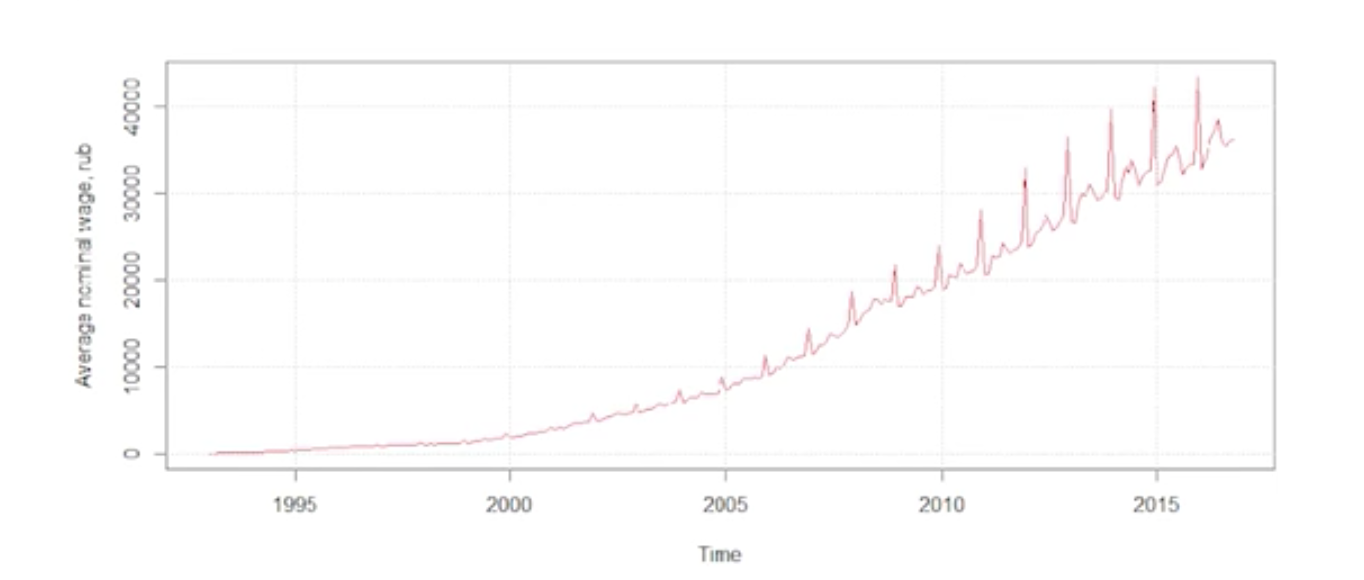
\includegraphics[totalheight=7cm]{main_part/timeline-payings.png}
% 	\caption{Пример временного ряда}
% 	\label{sec:purpose:payings}
% \end{figure}

% На данном рисунке видно, что, есть тренд к росту зарплат и пики, в декабре - месяце, где выдаются годовые премии. Длина ряда не является фиксированной величиной и может меняться, день, неделя, месяц, квартал, год. Сам по себе промежуток не имеет значения при прогнозировании.

% Задачей прогнозирования временных рядов является поиск функции F, которая будет будет зависеть от всей известной информации к моменту прогнозирования, который обозначается $ T $. На вход данная функция принимает все значения ряда, от $ Y_1$ до $ Y_t $. Также, функция принимает дополнительный параметр $ H $, который показывает насколько вперёд необходимо прогнозировать ряд. Параметр $h$ принимает значения от 1 до $ H $ ($ h \in {1, 2, ... H} $), где $ H $ называется горизонтом прогнозирования.

% Помимо прогнозов, которые представляют собой число, при прогнозировании полезно добавлять интервал, который показывает вероятность, с которой будет выполнено предсказание.
% Такой интервал называется предсказательным. 

% Предсказательный интервал - интервал, в котором предсказываемая величина окажется с вероятностью не меньше заданной. В данном случае, не стоит его путать с доверительным интервалом, который является случайным интервалом, для фиксированного неслучайного параметра. Предсказательный интервал является очень полезным инструментом, т.к. он показывает заказчику прогноза, насколько можно быть уверенным в произведённом прогнозе. И в данном случае важно, данную степень неуверенности квантифицировать.

% Как пример: в апреле 1997 в городе Гранд-Фокс, Северная Дакота, произошло наводнение. Город был защищён дамбой высотой 51 фут, согласно прогнозу, высота паводка должна была составить 49 футов, истинная же высота, оказалась 54. В результате этой ошибки было эвакуировано 75\% населения города и нанесён ущерб на несколько миллиардов долларов. На исторических данных, точность прогнозов метеорологической службы составляла +- 9 футов.

% Таким образом, выделим особенности задачи прогнозирования временных рядов:
% \begin{itemize}
% 	\item в классических задачах анализа данных предполагается независимость наблюдений;
% 	\item при прогнозировании временных рядов, прогноз строится на исторических данных.
% \end{itemize}

% В отличии от задач машинного обучения и статистики, где значения, как правило, являются простой выборкой, т.е. разные наблюдения, померенные на разных объектах, независимые одинаково распределённые. В то время как при прогнозировании временных рядов, данные устроены принципиально по другому - будущее зависит от прошлого, т.е. чем меньше прошлое похоже на шум, тем точнее можно будет сделать прогноз.

% Лучше всего, в машинном обучении, решаются задачи с учителем, т.е. есть определённом количество признаков и выходы, для данных признаков. В данном же случае, прогнозирования временных рядов, отсутсвуют $ x $-ы, т.е. отсутствуют признаки, есть только $y$-ки \cite{datamining_in_action}.

% \begin{figure}[h]
% \centering
% 	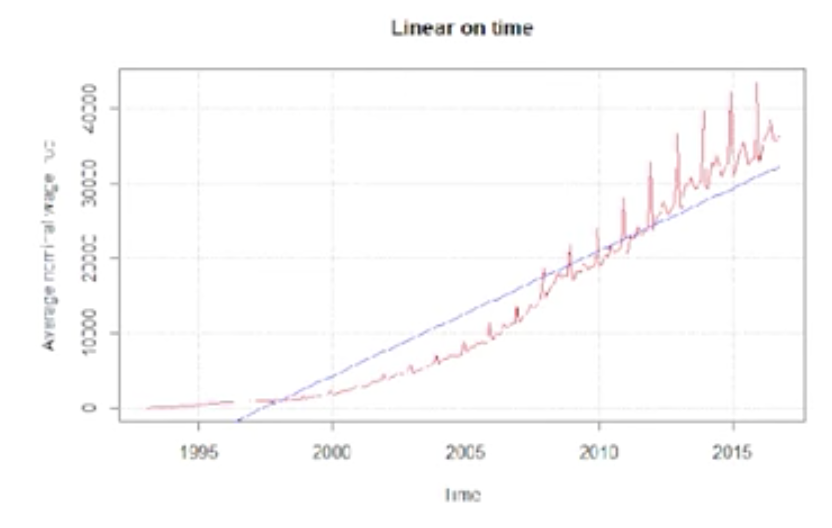
\includegraphics[totalheight=7cm]{main_part/linear-on-time.png}
% 	\caption{Применение методов машинного обучения (линейное)}
% 	\label{sec:purpose:linear}
% \end{figure}

% В данном рисунке видно, что предсказания (синяя линия) не будут достаточно точными, т.к. они явно не учитывают нешумовые всплески \cite{datamining_in_action}.

% \begin{figure}[h]
% \centering
% 	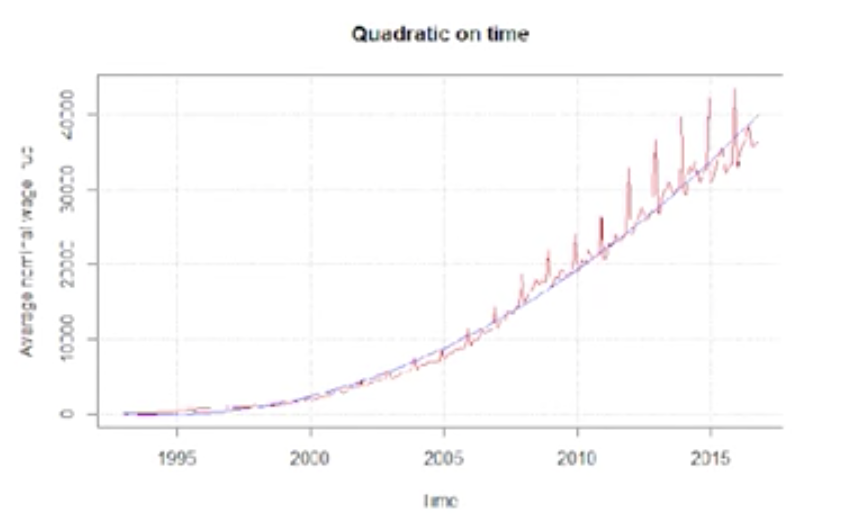
\includegraphics[totalheight=7cm]{main_part/quadratic-on-time.png}
% 	\caption{Применение методов машинного обучения (квадратичное)}
% 	\label{sec:purpose:quadratic}
% \end{figure}

% Также и применение квадратичной функции не приводит к точному предсказанию.

% Ключевая особенность временного ряда заключается в том, что соседние значения не независимы. Квантифицировать это можно с помощью автокорреляции. Автокорреляция, это корреляция ряда с самим собой, сдвинутым на определённое количество отсчётов. То количество, на которое мы сдвигаем отсчёт, называется \textit{лагом} автокорреляции. Автокорреляция меняет свои значения от -1 до 1, 1 означает идеальную линейную зависимость с положительным знаком, -1 - линейная зависимость с отрицательным, 0 - отсутствие линейной зависимости.

% Также необходимо рассмотреть компоненты временных рядов, т.е. то, из чего состоят ряды.

% \textit{Тренд} - плавное долгосрочное среднего изменения уровня ряда. Ряд может <<колебаться>> вокруг своего тренда.

% \textit{Сезонность} - циклические изменения уровня ряда с постоянным периодом. Например, если рассматриваются месячные ряды, то в них, скорее всего, будет годовая сезонность, т.е. то, что происходит в декабре этого года, будет похоже на то, что происходило в декабре предыдущего года.

% \textit{Цикл} - изменения уровня ряда с переменным периодом (например экономические циклы, периоды солнечной активности).

% \textit{Ошибка} - непрогнозируемая случайная компонента ряда.

% Ошибку, также, можно описать как то, что нельзя описать любыми другими компонентами ряда. Рассмотрим несколько примеров.

% В данном ряде можно рассмотреть тренд к падению количества контрактов сокровищницы США по дням \cite{datamining_in_action}.

% \begin{figure}[h]
% \centering
% 	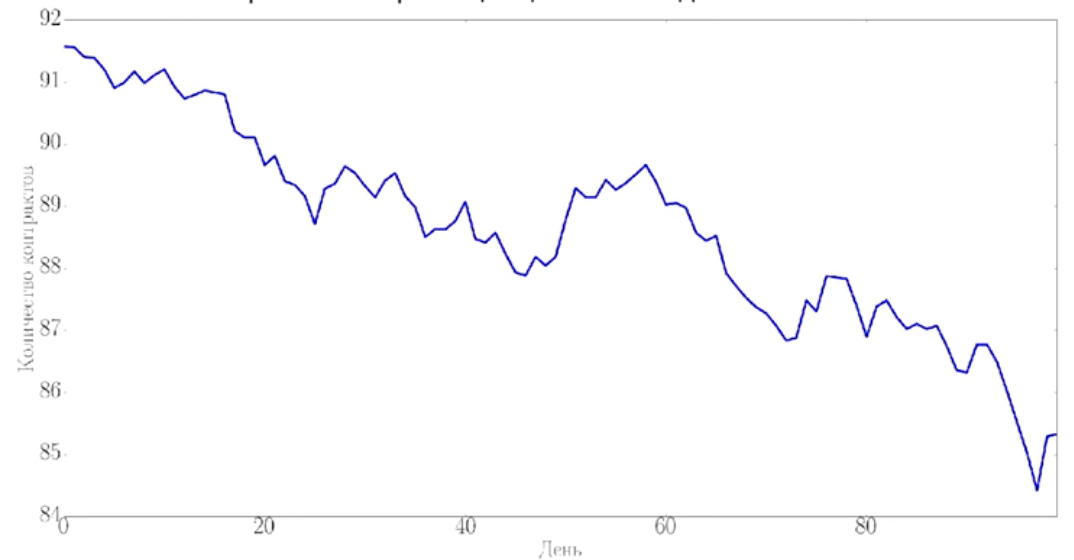
\includegraphics[totalheight=7cm]{main_part/usa-gold.png}
% 	\caption{Количества контрактов сокровищницы США}
% 	\label{sec:purpose:contracts}
% \end{figure}

% Это ряд, в котором можно отметить линейно понижающийся тренд. Можно сказать, что ряд совершает <<колебания>> вокруг своей линии тренда.

% Далее можно рассмотреть ряд с объёмами производства электричества в Австралии \cite{datamining_in_action}.

% \begin{figure}[h]
% \centering
% 	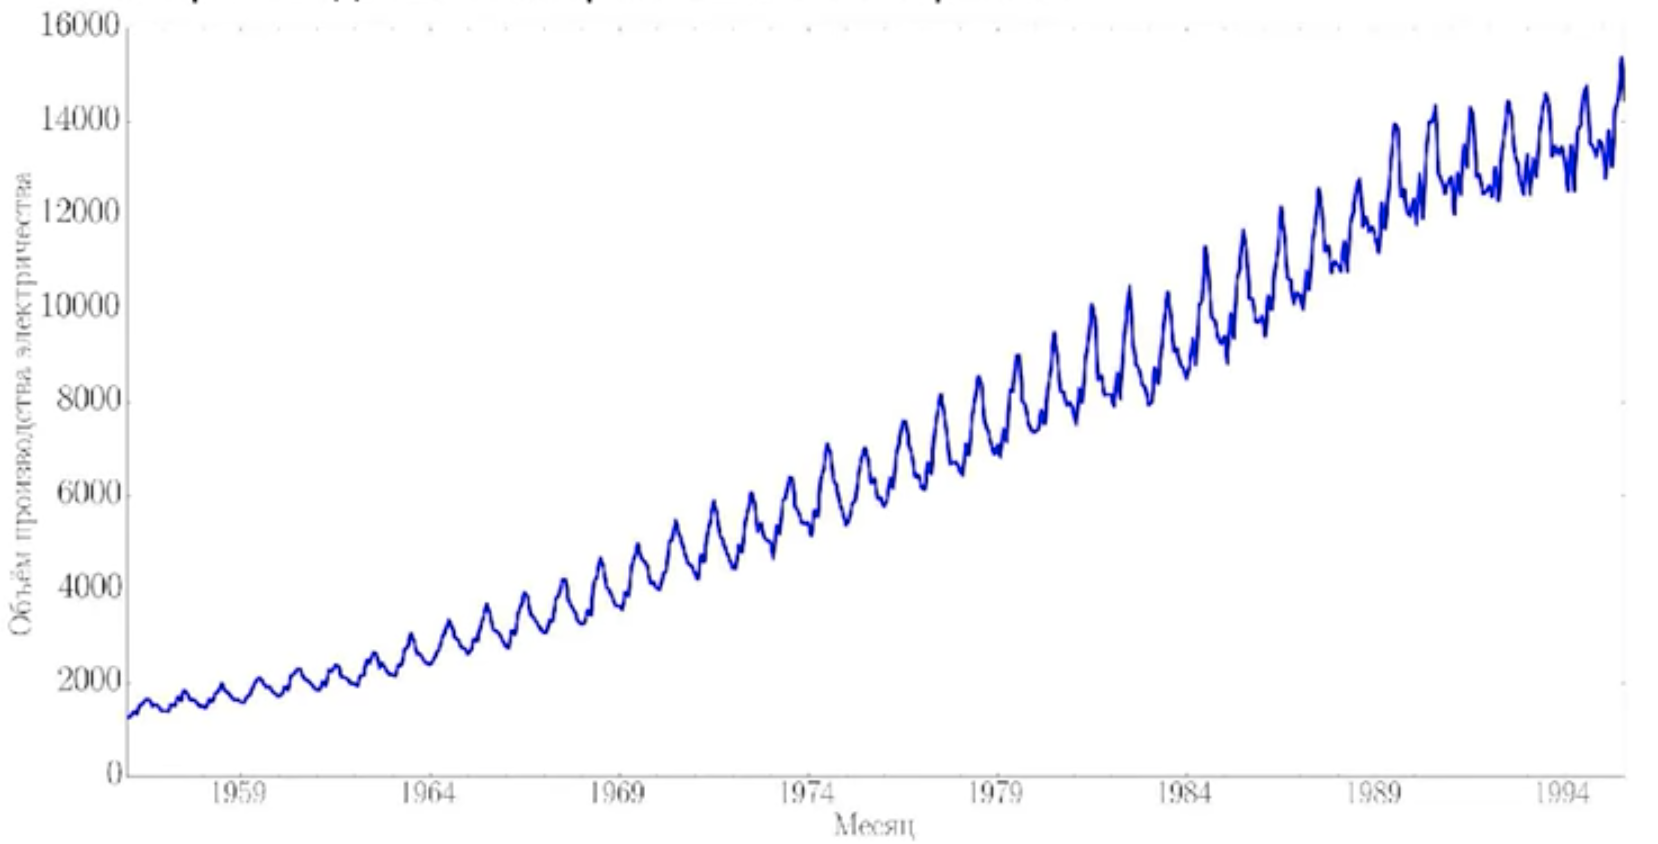
\includegraphics[totalheight=7cm]{main_part/australia-electricity.png}
% 	\caption{Объём производства электричества в Австралии}
% 	\label{sec:purpose:electricity}
% \end{figure}

% В данном ряде есть ярковыраженный повышающийся тренд и кроме того, сильная годовая сезонность. Хорошо видно, что на графике происходят колебания на середину лета - зиму в Австралии, с повышением потребления электричества.

% На следующем графике представлен временной ряд продажи жилых домов \cite{datamining_in_action}.

% \begin{figure}[h]
% \centering
% 	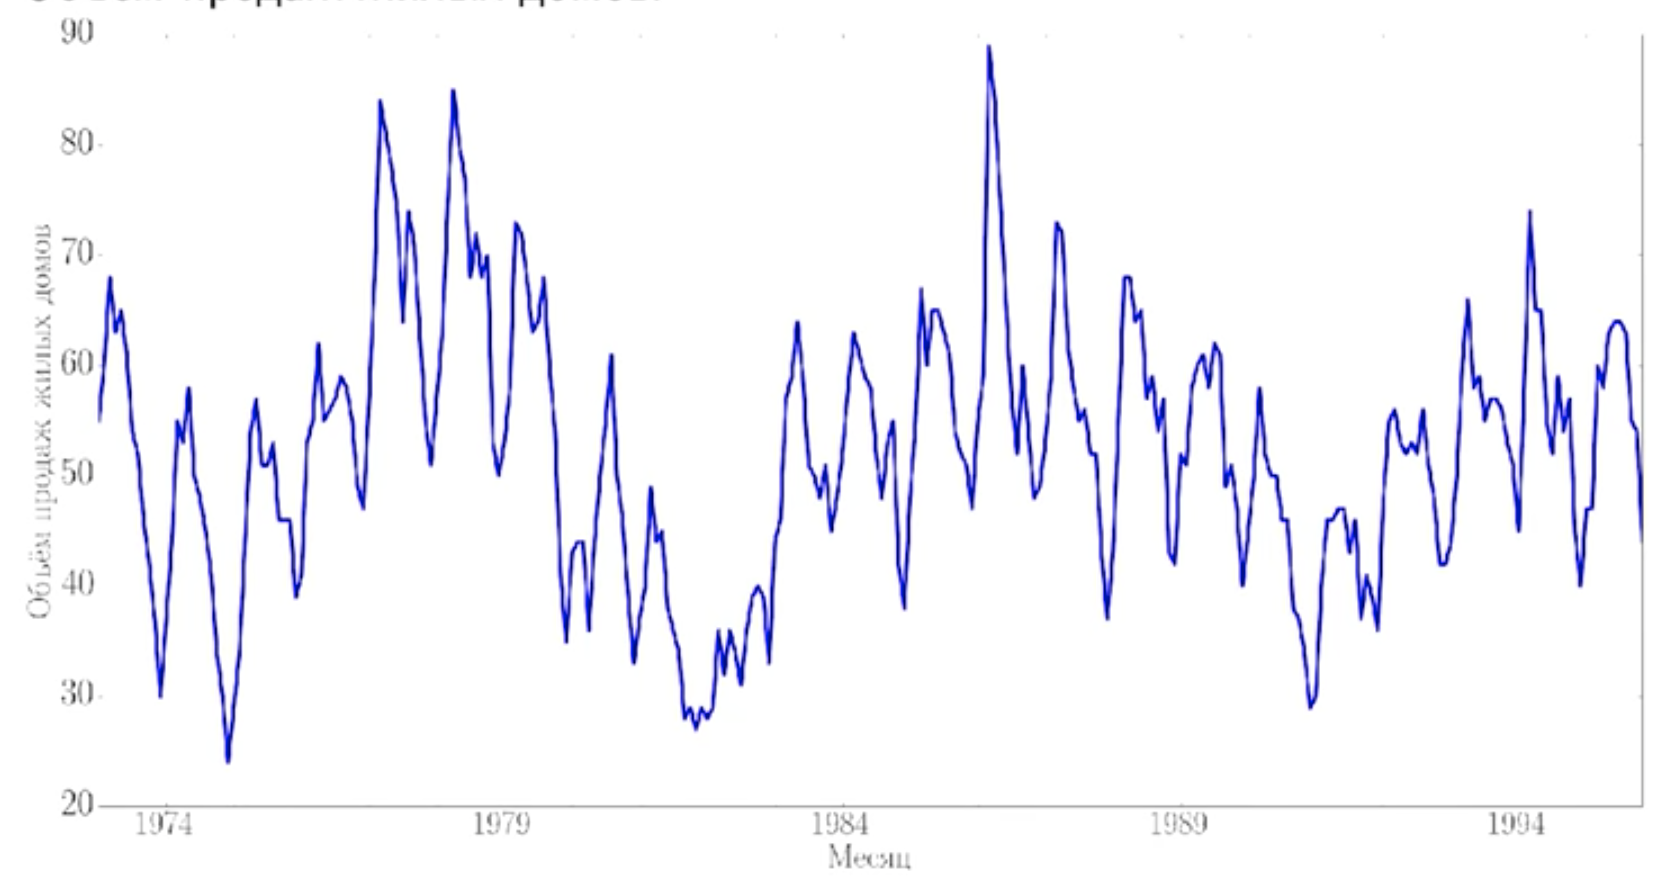
\includegraphics[totalheight=7cm]{main_part/house-sells.png}
% 	\caption{Объём продажи жилых домов в США}
% 	\label{sec:purpose:house-sells}
% \end{figure}

% На данном графике можно заметить годовую сезонность, длиной премерно равной году, и экономические циклы, которые можно отметить спадами и подъёмами объёмов продаж с нефиксированной временной длиной.




